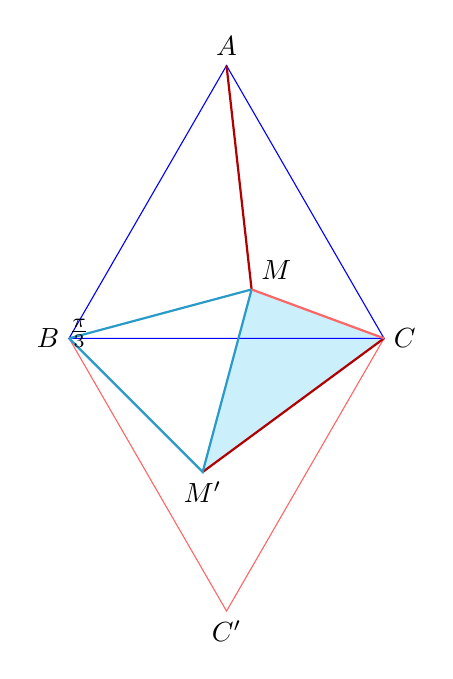
\begin{tikzpicture}[scale = 4]
      \draw (0,0) coordinate(B) node[left] {$B$}
        (1,0) coordinate(C) node[right]{$C$}
        (60:1) coordinate(A) node[above] {$A$}
        (-60:1) coordinate(C') node[below] {$C'$}
        (15:0.6) coordinate(M)node[above right]{$M$}
        (-45:0.6) coordinate(M')node[below]{$M'$};
      \fill [cyan,opacity=0.2] (C) -- (M) -- (M');
      \draw [blue] (B) -- (C) -- (A) -- cycle;
      \draw [red!60] (B) -- (C') -- (C);
      \draw [thick,red!70!black] (A) -- (M) (C) -- (M');
      \draw [thick,cyan!80!black] (B) -- (M)(M) -- (M') -- (B);
      \draw [thick,red!60] (C) -- (M);
      \tkzLabelAngle[pos=0.18](M',B,M){$\frac\pi3$}
      \tkzMarkAngle[cyan,size=0.1cm,mark=none](M',B,M)
    \end{tikzpicture}